\documentclass[12pt,a4paper]{article}
\usepackage[margin=1in]{geometry}
\usepackage{amsmath}
\usepackage{amsfonts}
\usepackage{amssymb}
\usepackage{graphicx}
\usepackage{hyperref}
\usepackage{url}
\usepackage{listings}
\usepackage{listings-rust}

\lstset{language=Rust, style=boxed}

\title{Cyber Physical Robots\\Term Project Progress Report II}
\author{Kanisorn Sangchai (ID: 6538020621)}
\date{October 3, 2025}

\begin{document}

\maketitle

\begin{abstract}
This report documents the second milestone of the Cyber-Physical Robots (CPR) project, which focuses on implementing communication protocols that allow robots within the same team to reach a consensus. At this stage, the robots are able to coordinate and agree on which pair should retrieve a given piece of gold, move to its location, and align themselves to face the same direction as their partner. The source code for this project is available at: \url{https://github.com/Kanisorn-S/CPR}
\end{abstract}

\section{Introduction}
This report documents the implementation of communication protocols for multi-robot coordination. The system enhances the simulation by enabling robots within the same team to reach consensus on specific tasks. Three protocols were implemented: one for identifying local clusters of robots, PAXOS for selecting the pair assigned to collect gold, and a simple request/acknowledgment mechanism for determining the robots’ facing direction.

\section{Communication Protocols}
For each communication protocol (excluding PAXOS), we first design the flow of messages based on the requirements. Then, before implementing, we validated our designs by modeling them as petri nets. We then verified that the desired goal markings were reachable and that no undesirable states could occur.

\subsection{\texttt{Local Cluster Identification}}
Before applying PAXOS to decide which pair of robots should retrieve a gold position, we first divide the robots into clusters based on the gold positions they are “eyeing.” At the start of the simulation, each robot would
\begin{enumerate}
    \item Observes its environment and selects the position with the highest amount of gold
    \item Broadcasts a simple message to all others containing the coordinates of the gold it has selected.
    \item After receiving all messages, it can determine which robots belong to its local cluster.
\end{enumerate}
This process is illustrated in Figure~\ref{fig:cluster-flow}.
Each cluster then applies PAXOS to agree on the pair that will collect the gold.

\begin{figure}
    \centering
    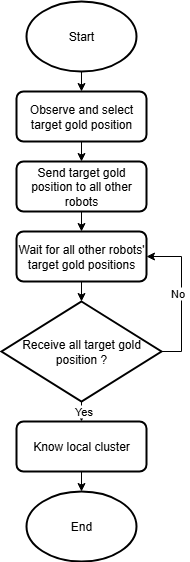
\includegraphics[width=0.2\linewidth]{images/cluster_flow.png}
    \caption{Flow Chart of the Local Cluster Identification Communication Protocol for each Robot}   
    \label{fig:cluster-flow}
\end{figure}

\subsubsection{Mathematical Formalism}

\begin{figure}[htbp]
    \centering
    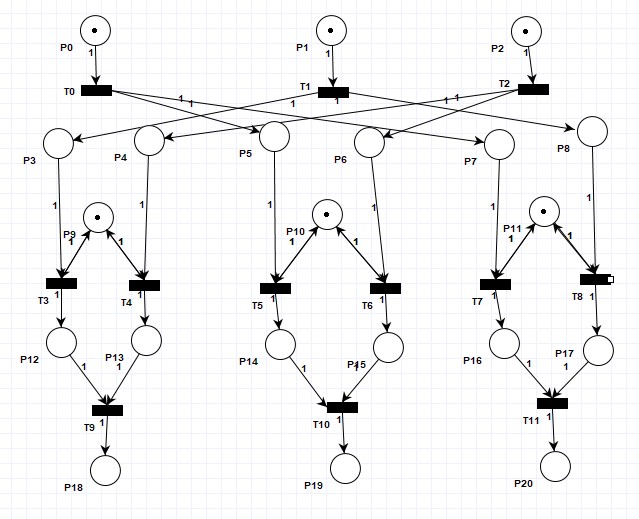
\includegraphics[width=0.8\linewidth]{images/cluster_petri.jpg}
    \caption{Petri Net of the Local Cluster Identification Communication Protocol}   
    \label{fig:cluster-petri}
\end{figure}

We modeled this communication protocol for three robots—A, B, and C—using a Petri net, shown in Figure~\ref{fig:cluster-petri}. Common Petri net patterns were applied in the model: synchronization was used to represent the requirement that a robot must know all other robots’ target positions before determining its local cluster, and conflict was used to capture the constraint that a robot may only read one message per simulation time step.

The mathematical formulation of the petri net, $PN_{\text{cluster}}$ shown in Figure~\ref{fig:cluster-petri} is as follow:
\begin{align*}
    PN_{\text{cluster}} &= (P_{\text{cluster}}, T_{\text{cluster}}, W_{\text{cluster}}, M_{0, \text{cluster}})
\end{align*}
Where
\begin{align*}
    P_{\text{cluster}} &= \{p_0, p_1, \ldots, p_{20}\} \\
    T_{\text{cluster}} &= \{t_0, t_1, \ldots, t_{11}\} \\
\end{align*}
importantly
\begin{align*}
    p_0 &\text{ is Robot A selects a target position} \\
    p_1 &\text{ is Robot B selects a target position} \\
    p_2 &\text{ is Robot C selects a target position} \\
    p_{18} &\text{ is Robot A knowing its local cluster} \\
    p_{19} &\text{ is Robot B knowing its local cluster} \\
    p_{20} &\text{ is Robot C knowing its local cluster} \\
\end{align*}
and ${\displaystyle W_{\text{cluster}}:(P_{\text{cluster}}\times T_{\text{cluster}})\cup (T_{\text{cluster}}\times P_{\text{cluster}})\to \mathbb {N} }$, which can also be represented by
\begin{align*}
    &W^{-}, \text{defined by } \forall p,t : W^{-}[p,t] = W(p, t) \\
    &W^{+}, \text{defined by } \forall p,t : W^{+}[p,t] = W(t, p) \\
    &W^{T} = -W^{-} + W^{+}
\end{align*}
The initial marking $M_{0, \text{cluster}}$ represents all robots, in this case 3, selecting a position with the highest amount of gold, and the target marking $M_{t, \text{cluster}}$ represents all robots knowing their local cluster.
\begin{align*}
    M_{0, \text{cluster}} = \begin{bmatrix}
        1 \\ 1 \\ 1 \\ 0 \\ \vdots \\ 0
    \end{bmatrix}_{21 \times 1}
    M_{t, \text{cluster}} = \begin{bmatrix}
        0 \\ \vdots \\ 0 \\ 1 \\ 1 \\ 1
    \end{bmatrix}_{21 \times 1}
\end{align*}
The full mathematical formalism is given in Appendix~\ref{app:cluster}.

From the petri net, we can see that the target marking $M_{t, \text{cluster}}$ is reachable from the initial marking $M_{0, \text{cluster}}$ by firing all transitions $t_0, t_1, \cdots, t_{11}$ in order.

\subsubsection{Software Implementation}
To implement this protocol in software, we make each robot follow the flow shown in Figure~\ref{fig:cluster-flow}. Firstly, the robot observes the environment and find the position with the most amount of gold then sends the coordinate to all other robots, as shown in Listing~\ref{lst:find-gold}
\begin{lstlisting}[float, caption={Robot Observes and Find where the most Gold is}, label={lst:find-gold}]
for observable_cell in self.observable_cells.iter() {
  let observed_cell = grid.get_cell(*observable_cell);
  if observed_cell.get_gold_amount().is_some() && !self.send_target {
    if observed_cell.get_gold_amount() > self.max_gold_seen {
      self.max_gold_seen = observed_cell.get_gold_amount();
      self.target_gold = Some(observed_cell.coord);
      self.message_to_send = Some(Message::new(
        self.id,
        MessageType::Simple,
        self.id as u32,
        MessageContent::Coord(Some(observed_cell.coord)),
      ));
    }
  }
}
// ...
self.send(self.message_to_send, self.receiver_ids);
\end{lstlisting}
Then the robot waits until it receives the target coordinate of all other robots, keeping track of robots that are targeting the same gold as itself, as shown in Listing~\ref{lst:find-local}. Once all coordinates are received, the robot would know its local cluster. This will need to be made more robust in the future.
\begin{lstlisting}[float, caption={Robot Receives Target Gold Coordinates and Keep Track of Local Cluster}, label={lst:find-local}]
match received_message {
  // ...
  MessageType::Simple => {
    if self.not_received_simple > 0 {
      self.not_received_simple -= 1;
      if self.target_gold.is_some() {
        match message.message_content {
          MessageContent::Coord(Some(coord)) => {
            if coord == self.target_gold {
              self.local_cluster.push(message.sender_id);
            }
          },
          _ => {}
        }
      }
    }
  },
  // ...
}

\end{lstlisting}

\subsection{\texttt{PAXOS}}
After splitting the robots into local clusters according to their targeted gold positions, PAXOS is employed within each cluster to achieve consensus on the pair of robots designated to move to the target location and attempt to retrieve the gold.

\subsubsection{Software Implementation}
The PAXOS implemented is based on the PAXOS taught in class. In our simulation, all robots will assume the role of proposer, acceptor, and learner. Once a robot knows its local cluster, it would send a \texttt{PrepareRequest} to all other robots in its local cluster to propose a pair of robots to attempt to retrieve the targeted gold, as shown in Listing~\ref{lst:paxos-init}.
\begin{lstlisting}[float, caption={Robot Sends a \texttt{PrepareRequest} to Propose a Robot Pairing}, label={lst:paxos-init}]
if (!self.send_pair_request) {
  let mut rng = rand::rng();
  let pair_id = self.local_cluster.choose(&mut rng);
  if pair_id.is_some() {
    self.message_to_send = Some(Message::new(
      self.id,
      MessageType::PrepareRequest,
      self.id as u32,
      MessageContent::Pair(self.id, *pair_id)),
    );
    self.send(self.message_to_send, self.local_cluster);
    self.majority = (self.local_cluster.len() / 2) as u8;
    self.send_pair_request = true;
  }
}
\end{lstlisting}
At each simulation step, every robot receives a single message and responds according to the rules of the PAXOS algorithm. 

\begin{itemize}


\item Upon receiving a \texttt{PrepareRequest}, the robot first checks whether it has already promised another message. If no promise has been made, it accepts the request by issuing a promise and replying with a \texttt{PrepareResponse}. If a promise exists, the robot compares the id of the received request with that of its current promise. If the new id is higher, the robot updates its promise to the new request and replies with a \texttt{PrepareResponse}, including the value of the previously promised message. If the new id is not higher, the robot ignores the request. This process is illustrated in Figure~\ref{fig:prepare-request}, and the corresponding implementation is shown in Listing~\ref{lst:prepare-request}.

\begin{figure}
    \centering
    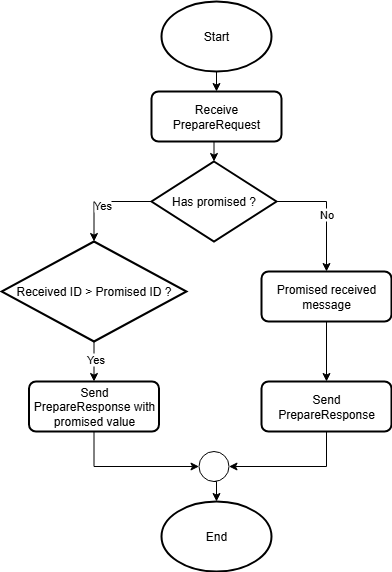
\includegraphics[width=0.5\linewidth]{images/prepare_request.png}
    \caption{Flow Chart of Robot Responding to a \texttt{PrepareRequest}}   
    \label{fig:prepare-request}
\end{figure}

\begin{lstlisting}[float, caption={Robot Receives a \texttt{PrepareRequest}}, label={lst:prepare-request}]
match received_message.msg_type {
  MessageType::PrepareRequest => {
    match self.promised_message {
      Some(promised_message) => {
        if (promised_message.id < message.id) {
          self.promised_message = Some(Message::new(
            promised_message.sender_id,
            promised_message.msg_type,
            message.id,
            promised_message.message_content,
          ));
          let piggyback_msg = Message::new(
            self.id,
            MessageType::PrepareResponse,
            promised_message.id,
            promised_message.message_content,
          );
          self.send(piggyback_msg, vec![message.sender_id]);
        } 
      },
      None => {
        self.promised_message = Some(message);
        let promised = Message::new(
          self.id,
          MessageType::PrepareResponse,
          message.id,
          message.message_content,
        );
        self.send(promised, vec![message.sender_id]);
      }
    }
  },
  // ...
}
\end{lstlisting}

\item Upon receiving a \texttt{PrepareResponse}, the robot increments its promise count. It then checks whether the response contains a piggybacked value. If so, the robot updates its proposed message to match the piggybacked value that comes with the highest message id. Once the robot receives a majority of promises, the robot sends an \texttt{AcceptRequest} to all other robots in its local cluster. This process is illustrated in Figure~\ref{fig:prepare-response}, and the corresponding implementation is provided in Listing~\ref{lst:prepare-response}.

\begin{figure}
    \centering
    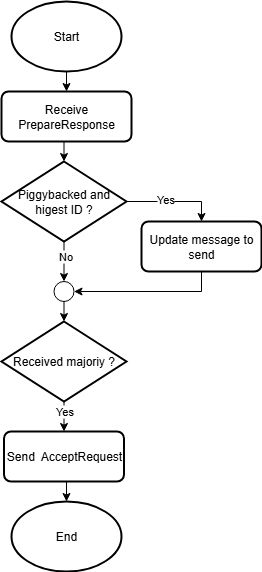
\includegraphics[width=0.5\linewidth]{images/prepare_response.png}
    \caption{Flow Chart of Robot Responding to a \texttt{PrepareResponse}}   
    \label{fig:prepare-response}
\end{figure}

\begin{lstlisting}[float, caption={Robot Receives a \texttt{PrepareResponse}}, label={lst:prepare-response}]
match received_message.msg_type {
  MessageType::PrepareResponse => {
    self.promise_count += 1;
    if (message.id == self.message_to_send.id) {
      if (self.promise_count > self.majority) {
        self.reached_majority = true;
        let message_to_send = self.message_to_send;
        let accept_request_msg = Message::new(
          self.id,
          MessageType::AcceptRequest,
          message_to_send.id,
          message_to_send.message_content,
        );
        self.send(accept_request_msg, self.local_cluster);
      }
    } else {
      self.piggybacked = true;
      // Update highest piggyback ID
      if (message.id > self.max_piggyback_id_seen) {
        self.max_piggyback_id_seen = message.id;
        let message_to_send = self.message_to_send;
        let new_message_to_send = Message::new(
          self.id,
          MessageType::AcceptRequest,
          message_to_send.id,
          message.message_content,
        );
        self.message_to_send = Some(new_message_to_send);
      }
      // Check majority
      if (self.promise_count > self.majority) {
        self.reached_majority = true;
        self.send(self.message_to_send, self.local_cluster);
      }
    }
  },
  // ...
}
\end{lstlisting}

\item Upon receiving an \texttt{AcceptRequest}, the robot checks whether the request’s id is greater than or equal to its promised id. If so, it accepts the message and replies with an \texttt{Accepted}. If the id is smaller, the robot ignores the request. This process is illustrated in Figure~\ref{fig:accept-request}, and the corresponding implementation is shown in Listing~\ref{lst:accept-request}.

\begin{figure}
    \centering
    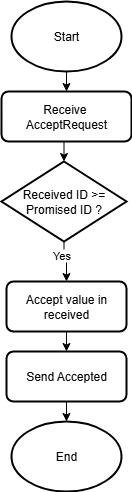
\includegraphics[width=0.2\linewidth]{images/accept_request.png}
    \caption{Flow Chart of Robot Responding to a \texttt{AcceptRequest}}   
    \label{fig:accept-request}
\end{figure}

\begin{lstlisting}[float, caption={Robot Receives a \texttt{AcceptRequest}}, label={lst:accept-request}]
match received_message.msg_type {
  MessageType::AcceptRequest => {
    match self.promised_message {
      Some(promised_message) => {
        if (promised_message.id <= message.id) {
          self.accepted = true;
          self.promised_message = Some(message);
          let accepted_msg = Message::new(
            self.id,
            MessageType::Accepted,
            message.id,
            message.message_content,
          );
          self.send(accepted_msg, vec![message.sender_id]);
        }
      },
      None => {}
    }
  },
  // ...
}
\end{lstlisting}

\item Upon receiving an \texttt{Accepted}, the robot increments its accept count. Once a majority of acceptances is reached, the robot concludes that consensus has been achieved on its proposed value and updates its own consensus accordingly. It then broadcasts a \texttt{Confirm} message to all other robots in its local cluster, allowing them to update their consensus as well. This process is illustrated in Figure~\ref{fig:accepted}, and the corresponding implementation is shown in Listing~\ref{lst:accepted}.

\begin{figure}
    \centering
    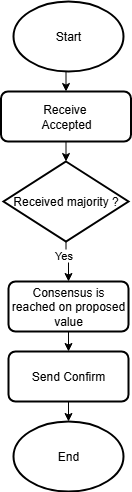
\includegraphics[width=0.2\linewidth]{images/accepted.png}
    \caption{Flow Chart of Robot Responding to a \texttt{Accepted}}   
    \label{fig:accepted}
\end{figure}

\begin{lstlisting}[float, caption={Robot Receives a \texttt{Accepted}}, label={lst:accepted}]
match received_message.msg_type {
  MessageType::Accepted => {
    self.accept_count += 1;
    if (self.accept_count > self.majority) {
      self.set_consensus(message.message_content);
      self.promised_message = Some(message);
      self.send(Message::new(
        self.id,
        MessageType::Confirm,
        self.id as u32,
        message.message_content,
      ), self.local_cluster);
    }
  },
  // ...
}
\end{lstlisting}

\item Upon receiving a \texttt{Confirm}, the robot updates its consensus value. This corresponds to the role of the learner in PAXOS, which adopts the value that has been agreed upon.

\end{itemize}

A single round of basic PAXOS would then be complete, meaning if a robot isn't able to get a consensus on its desired robot pairing, it would not try and resend a \texttt{PrepareRequest} with a higher id.

\subsection{\texttt{Direction Selection}}
After a local cluster reaches consensus on the two robots designated to collect the targeted gold, the selected robots proceed to the gold’s location. To synchronize their actions and ensure the gold is transported successfully without being dropped, the two robots must first agree on a common facing direction. Once aligned, they can use the same path planner to generate a route to the deposit point. Because they are at the same position and share the same orientation, both robots will receive identical action sequences, guaranteeing stable transport of the gold. The agreement on facing direction is achieved by having each robot follow the process illustrated in Figure~\ref{fig:direction-flow}

\begin{figure}
    \centering
    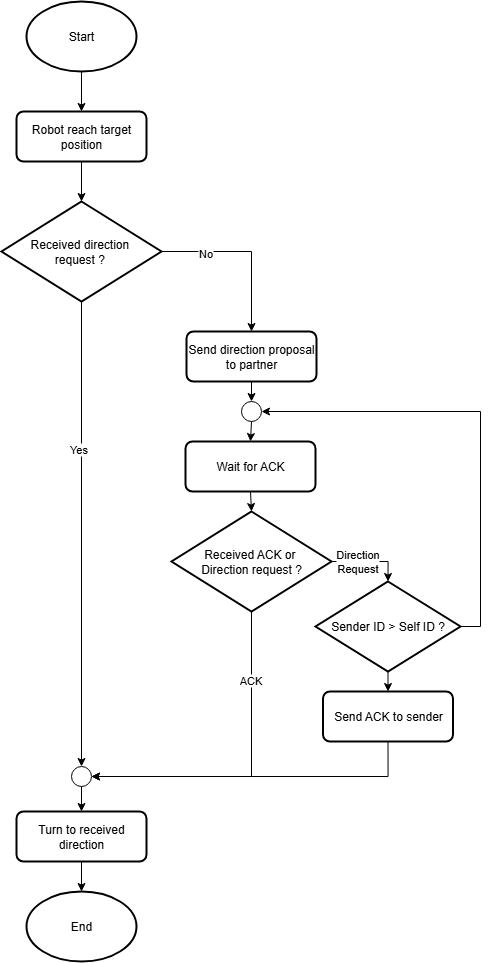
\includegraphics[width=0.5\linewidth]{images/direction_flow.png}
    \caption{Flow Chart of the Direction Selection Communication Protocol for each Robot}   
    \label{fig:direction-flow}
\end{figure}

\subsubsection{Mathematical Formalism}

\begin{figure}[htbp]
    \centering
    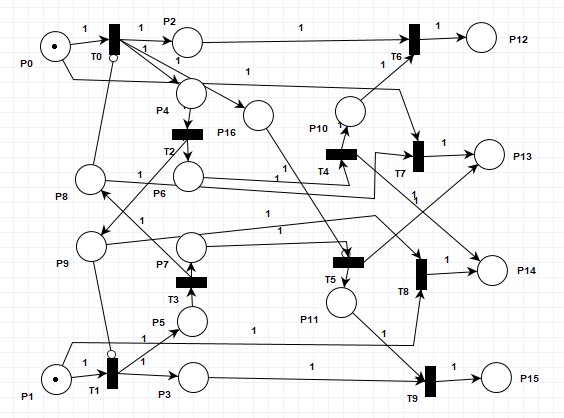
\includegraphics[width=0.8\linewidth]{images/direction_petri.jpg}
    \caption{Petri Net of the Local Cluster Identification Communication Protocol}   
    \label{fig:direction-petri}
\end{figure}

We modeled this communication protocol for two robots A and B, using a Petri net, shown in Figure~\ref{fig:direction-petri}. Common Petri net patterns were applied in the model: synchronization was used to represent the requirement that a robot must receive and ACK before confirming its direction, and priority was used by using the inhibitor arc.

The mathematical formulation of the petri net, $PN_{\text{direction}}$ shown in Figure~\ref{fig:direction-petri} is as follow:
\begin{align*}
    EPN_{\text{direction}} &= (P_{\text{direction}}, T_{\text{direction}}, W_{\text{direction}}, Inh_{direction}, M_{0, \text{direction}})
\end{align*}
Where
\begin{align*}
    P_{\text{direction}} &= \{p_0, p_1, \ldots, p_{15}\} \\
    T_{\text{direction}} &= \{t_0, t_1, \ldots, t_{9}\} \\
\end{align*}
importantly
\begin{align*}
    p_0 &\text{ is Robot A is at target location} \\
    p_1 &\text{ is Robot B is at target location} \\
    p_{12} &\text{ is \textbf{Robot A selects} direction} \\
    p_{13} &\text{ is \textbf{Robot A follows} Robot B} \\
    p_{14} &\text{ is \textbf{Robot B follows} Robot A} \\
    p_{15} &\text{ is \textbf{Robot B selects} direction} \\
\end{align*}
${\displaystyle W_{\text{direction}}:(P_{\text{direction}}\times T_{\text{direction}})\cup (T_{\text{direction}}\times P_{\text{direction}})\to \mathbb {N} }$, which can also be represented by
\begin{align*}
    &W^{-}, \text{defined by } \forall p,t : W^{-}[p,t] = W(p, t) \\
    &W^{+}, \text{defined by } \forall p,t : W^{+}[p,t] = W(t, p) \\
    &W^{T} = -W^{-} + W^{+}
\end{align*}
and ${\displaystyle Inh_{\text{direction}}:P_{\text{direction}}\times T_{\text{direction}}\to \mathbb {N} }$.

The initial marking $M_{0, \text{direction}}$ represents both robots arriving at the target location, the target marking $M_{t, \text{direction}}$ represents both robots agreeing on who chooses the direction, and the undesired marking $M_{u, \text{direction}}$ represents the robots disagreeing on who chooses the direction.
\begin{align*}
    M_{0, \text{direction}} = \begin{bmatrix}
        1 \\ 1 \\ 0 \\ 0 \\ \vdots \\ 0
    \end{bmatrix}_{16 \times 1}
    M_{t, \text{direction}} = \begin{bmatrix}
        0 \\ \vdots \\ 1 \\ 0 \\ 1 \\ 0
    \end{bmatrix}_{16 \times 1} \text{or } 
    \begin{bmatrix}
        0 \\ \vdots \\ 0 \\ 1 \\ 0 \\ 1
    \end{bmatrix}_{16 \times 1}
    M_{u, \text{direction}} = \begin{bmatrix}
        0 \\ \vdots \\ 1 \\ 0 \\ 0 \\ 1
    \end{bmatrix}_{16 \times 1} \text{and } 
    \begin{bmatrix}
        0 \\ \vdots \\ 0 \\ 1 \\ 1 \\ 0
    \end{bmatrix}_{16 \times 1}
\end{align*}
The full mathematical formalism is given in Appendix~\ref{app:direction}.

From the petri net, we verify that the target marking $M_{t, \text{direction}}$ is reachable and the undesired marking $M_{u, \text{direction}}$ is unreachable from the initial marking $M_{0, \text{direction}}$ by using PIPE (\url{https://github.com/sarahtattersall/PIPE}), a petri net modeler. After creating the petri net in PIPE, we used the GSPN analysis tool to analyze the petri net. The analysis result, as shown in Figure~\ref{fig:pipe-analysis}, confirms that the target marking is reachable and the undesired marking is unreachable. 

\begin{figure}
    \centering
    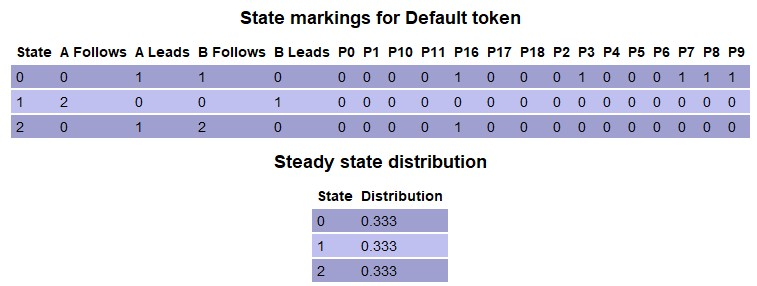
\includegraphics[width=\linewidth]{images/pipe_analysis.jpg}
    \caption{Analysis Result from PIPE}   
    \label{fig:pipe-analysis}
\end{figure}

\subsubsection{Software Implementation}
To implement this protocol in software, we make each robot follow the flow shown in Figure~\ref{fig:direction-flow}. Firstly, once the robot reaches the target location, it would send a request message to its partner to propose a direction, as shown in Listing~\ref{lst:direction-init}

\begin{lstlisting}[float, caption={Robot Sends Direction \texttt{Request}}, label={lst:direction-init}]
if self.current_coord == self.target_gold && !self.received_direction {
  if self.pre_pickup_pair_id.is_some() {
    let propose_direction;
    match rand::random_range(1..5) {
      1 => propose_direction = Direction::Right,
      2 => propose_direction = Direction::Left,
      3 => propose_direction = Direction::Up,
      4 => propose_direction = Direction::Down,
      _ => propose_direction = Direction::Right,
    }
    self.send(Message::new(
      self.id,
      MessageType::Request,
      self.id as u32,
      MessageContent::Direction(propose_direction),
      ), vec![self.pre_pickup_pair_id.unwrap()]);
    self.sent_direction_request = true;
  }
}
\end{lstlisting}

Upon receiving a direction \texttt{Request}, if the robot has not yet reached the target location, it would follow the request by adding the \texttt{TURN} action to its action queue, then replying with an \texttt{ACK} message, as shown in Listing~\ref{lst:direction-request}.

\begin{lstlisting}[float, caption={Robot Receives Direction \texttt{Request}}, label={lst:direction-request}]
match received_message {
  // ...
  MessageType::Request => {
    if self.id < message.sender_id || 
    self.current_coord != self.target_gold {
      self.send(Message::new(
        self.id,
        MessageType::Ack,
        self.id as u32,
        message.message_content,
      ), vec![message.sender_id]);
      match message.message_content {
        MessageContent::Direction(direction) => {
          self.planned_actions.push(Turn(direction));
          self.received_direction = true;
        },
        _ => {}
      }
    }
  },
  // ...
}
\end{lstlisting}

Finally, once the robot receives an \texttt{ACK}, it would confirm the direction by adding the \texttt{TURN} action to its action queue, as shown in Listing~\ref{lst:direction-ack}.

\begin{lstlisting}[float, caption={Robot Receives \texttt{ACK}}, label={lst:direction-ack}]
match received_message {
  // ...
  MessageType::Ack => {
    match message.message_content {
      MessageContent::Direction(direction) => {
        self.planned_actions.push(Turn(direction));
      },
      _ => {}
    }
  },
  // ...
}
\end{lstlisting}
 
\section{Current Progress and Results}
\begin{enumerate}
    \item \textbf{Complete Path Planning Algorithm:} A simple path planning algorithm to generate a sequence of action based on a robot's current and target position was implemented but was not mentioned in this report.
    \item \textbf{Communication Protocols:} Three communication protocols were implemented: one for identifying local clusters of robots, PAXOS for selecting the pair assigned to collect gold, and a simple request/acknowledgment mechanism for determining the robots’ facing direction.
    \item \textbf{Petri Net Simulation:} Petri nets were used to model and validate the communication protocols before implementation. The models confirmed that the desired states were reachable and that no undesirable states could occur.
\end{enumerate}

\section{Future Work}
\begin{enumerate}
    \item \textbf{Add Exploration} Currently, the robots rely on its initial observation to select a target gold position; therefore, if a robot is spawned facing a wall, it would simply have no target gold position. Adding exploration would allow the robots to find more gold positions.
    \item \textbf{Implement Random Message Arrival Time} Currently, each robot receives a random message from a list of available messages, meaning if a message is available, the robot would receive it immediately. Implementing random message arrival time would make the simulation more realistic.
\end{enumerate}


\section{Conclusion}
The second milestone is completed. The robots are now able to coordinate and agree on which pair should retrieve a given piece of gold, move to its location, and align themselves to face the same direction as their partner. 

\newpage
\appendix
\section{\texorpdfstring{Complete Mathematical Formulation for \\ \texttt{Local Cluster Identification}}{Complete Mathematical Formulation for Local Cluster Identification}}
\label{app:cluster}

\begin{align*}
    PN_{\text{cluster}} &= (P_{\text{cluster}}, T_{\text{cluster}}, W_{\text{cluster}}, M_{0, \text{cluster}})
\end{align*}
Where
\begin{align*}
    P_{\text{cluster}} &= \{p_0, p_1, \ldots, p_{20}\} \\
    T_{\text{cluster}} &= \{t_0, t_1, \ldots, t_{11}\} \\
\end{align*}
\begin{align*}
    p_0  &\text{ is A selects a target position}              & p_{12} &\text{ is A knows B's target position} \\
    p_1  &\text{ is B selects a target position}              & p_{13} &\text{ is A knows C's target position} \\
    p_2  &\text{ is C selects a target position}              & p_{14} &\text{ is B knows A's target position} \\
    p_3  &\text{ is B sent message to A}                     & p_{15} &\text{ is B knows C's target position} \\
    p_4  &\text{ is C sent message to A}                     & p_{16} &\text{ is C knows A's target position} \\
    p_5  &\text{ is A sent message to B}                     & p_{17} &\text{ is C knows B's target position} \\
    p_6  &\text{ is C sent message to B}                     & p_{18} &\text{ is A knows its local cluster} \\
    p_7  &\text{ is A sent message to C}                     & p_{19} &\text{ is B knows its local cluster} \\
    p_8  &\text{ is B sent message to C}                     & p_{20} &\text{ is C knows its local cluster} \\
    p_9  &\text{ is A can receive one message at a time}      &        & \\
    p_{10}&\text{ is B can receive one message at a time}     &        & \\
    p_{11} &\text{ is C can receive one message at a time}    &        & \\
\end{align*}
\begin{align*}
    t_0  &\text{ is A sends its target position}              & t_{6} &\text{ is B receives C's target position} \\
    t_1  &\text{ is B sends its target position}              & t_{7} &\text{ is C receives A's target position} \\
    t_2  &\text{ is C sends its target position}              & t_{8} &\text{ is C receives B's target position} \\
    t_3  &\text{ is A receives B's target position}                     & t_{9} &\text{ is A works out its local cluster} \\
    t_4  &\text{ is A receives C's target position}                     & t_{10} &\text{ is B works out its local cluster} \\
    t_5  &\text{ is B receives A's target position}                     & t_{11} &\text{ is C works out its local cluster} \\
\end{align*}

For input places and transitions,
\begin{align*}
  W_{\text{cluster}}(p_i, t_j) = 1 \text{ for } (i, j) \in 
\{&(0, 0), (1, 1), (2, 2), (3, 3), (4, 4), \\
  &(5, 5), (6, 6), (7, 7), (8, 8), (9, 3), \\
  &(9, 4), (10, 5), (10, 6), (11, 7), (11, 8), \\
  &(12, 9), (13, 9), (14, 10), (15, 10), (16, 11), (17, 11)\}
\end{align*}

For output places and transitions,
\begin{align*}
  W_{\text{cluster}}(t_i, p_j) = 1 \text{ for } (i, j) \in 
\{&(0, 5), (0, 7), (1, 3), (1, 8), (2, 4), \\
  &(2, 6), (3, 12), (4, 13), (5, 14), (6, 15), \\
  &(7, 16), (8, 17), (9, 18), (10, 19), (11, 20)\}
\end{align*}
The initial marking $M_{0, \text{cluster}}$ represents all robots, in this case 3, selecting a position with the highest amount of gold, and the target marking $M_{t, \text{cluster}}$ represents all robots knowing their local cluster.
\begin{align*}
    M_{0, \text{cluster}} = \begin{bmatrix}
        1 \\ 1 \\ 1 \\ 0 \\ \vdots \\ 0
    \end{bmatrix}_{21 \times 1}
    M_{t, \text{cluster}} = \begin{bmatrix}
        0 \\ \vdots \\ 0 \\ 1 \\ 1 \\ 1
    \end{bmatrix}_{21 \times 1}
\end{align*}

\section{\texorpdfstring{Complete Mathematical Formulation for \\ \texttt{Direction Selection}}{Complete Mathematical Formulation for Direction Selection}}
\label{app:direction}

\begin{align*}
    EPN_{\text{direction}} &= (P_{\text{direction}}, T_{\text{direction}}, W_{\text{direction}}, Inh_{\text{direction}}, M_{0, \text{direction}})
\end{align*}
Where
\begin{align*}
    P_{\text{direction}} &= \{p_0, p_1, \ldots, p_{15}\} \\
    T_{\text{direction}} &= \{t_0, t_1, \ldots, t_{9}\} \\
\end{align*}
\begin{align*}
    p_0  &\text{ is A is at target location}              & p_{8} &\text{ is A received \texttt{Request} from B} \\
    p_1  &\text{ is B is at target location}              & p_{9} &\text{ is B received \texttt{Request} from A} \\
    p_2  &\text{ is A waiting for \texttt{ACK}}              & p_{10} &\text{ is A received \texttt{ACK} from B} \\
    p_3  &\text{ is B waiting for \texttt{ACK}}                     & p_{11} &\text{ is B received \texttt{ACK} from A} \\
    p_4  &\text{ is A sent \texttt{Request} to B}                     & p_{12} &\text{ is A selects direction} \\
    p_5  &\text{ is B sent \texttt{Request} to A}                     & p_{13} &\text{ is A follows B} \\
    p_6  &\text{ is A received \texttt{Request} from B}                     & p_{14} &\text{ is B follows A} \\
    p_7  &\text{ is B received \texttt{Request} from A}                     & p_{15} &\text{ is B selects direction} \\
\end{align*}
\begin{align*}
    t_0  &\text{ is A sends \texttt{Request} to B}              & t_{5} &\text{ is A \texttt{ACK} B's \texttt{Request}} \\
    t_1  &\text{ is B sends \texttt{Request} to A}              & t_{6} &\text{ is A decides to choose direction} \\
    t_2  &\text{ is B receives A's \texttt{Request}}              & t_{7} &\text{ is A decides to follow B} \\
    t_3  &\text{ is A receives B's \texttt{Request}}                & t_{8} &\text{ is B decides to follow A} \\
    t_4  &\text{ is B \texttt{ACK} A's \texttt{Request}}                     & t_{9} &\text{ is B decides to choose direction} \\
\end{align*}

For input places and transitions,
\begin{align*}
  W_{\text{direction}}(p_i, t_j) = 1 \text{ for } (i, j) \in 
\{&(0, 0), (1, 1), (4, 2), (5, 3), (6, 4), \\
  &(7, 5), (2, 6), (10, 6), (0, 7), (8, 7), \\
  &(1, 8), (9, 8), (3, 9), (11, 9)\}
\end{align*}

For output places and transitions,
\begin{align*}
  W_{\text{direction}}(t_i, p_j) = 1 \text{ for } (i, j) \in 
\{&(0, 2), (0, 4), (0, 16), (1, 3), (1, 5), \\
  &(2, 6), (2, 9), (3, 7), (3, 8), (4, 10), \\
  &(4, 14), (5, 11), (5, 13), (6, 12), (7, 13) \\
  &(8, 14), (9, 15) \}
\end{align*}

For inhibitor arcs,
\begin{align*}
  Inh(p_i, t_j) = 1 \text{ for } (i, j) \in 
\{&(8, 0), (9, 1), (16, 5)\}
\end{align*}
The initial marking $M_{0, \text{direction}}$ represents both robots arriving at the target location, the target marking $M_{t, \text{direction}}$ represents both robots agreeing on who chooses the direction, and the undesired marking $M_{u, \text{direction}}$ represents the robots disagreeing on who chooses the direction.
\begin{align*}
    M_{0, \text{direction}} = \begin{bmatrix}
        1 \\ 1 \\ 0 \\ 0 \\ \vdots \\ 0
    \end{bmatrix}_{16 \times 1}
    M_{t, \text{direction}} = \begin{bmatrix}
        0 \\ \vdots \\ 1 \\ 0 \\ 1 \\ 0
    \end{bmatrix}_{16 \times 1} \text{or } 
    \begin{bmatrix}
        0 \\ \vdots \\ 0 \\ 1 \\ 0 \\ 1
    \end{bmatrix}_{16 \times 1}
    M_{u, \text{direction}} = \begin{bmatrix}
        0 \\ \vdots \\ 1 \\ 1 \\ 0 \\ 0
    \end{bmatrix}_{16 \times 1} \text{and } 
    \begin{bmatrix}
        0 \\ \vdots \\ 0 \\ 0 \\ 1 \\ 1
    \end{bmatrix}_{16 \times 1}
\end{align*}

\end{document}